\begin{figure}[htbp]
    \centering
    \begin{graybox}
    \makebox[1.5cm]{\textbf{GT}}\hspace{0.2cm}
    \makebox[3.02cm]{\textbf{IF-TONIR}}\hspace{0.2cm}
    \makebox[3.02cm]{\textbf{w/o point properties}}\hspace{0.2cm}
    \makebox[3.02cm]{\textbf{w/o positional encoding}}\hspace{0.2cm}
    \makebox[3.02cm]{\textbf{w/o physical fields}}
    \\
    
\includegraphics[width=1.5cm,height=1.5cm]{figs/ablation/27054-gt.png}\hspace{0.2cm}
    
\includegraphics[width=1.5cm,height=1.5cm]{figs/ablation/27054-pred.png}\hspace{0.02cm}
    
\includegraphics[width=1.5cm,height=1.5cm]{figs/ablation/strain-27054.png}\hspace{0.2cm}
    
\includegraphics[width=1.5cm,height=1.5cm]{figs/ablation/27054-wo-pp.png}\hspace{0.02cm}
    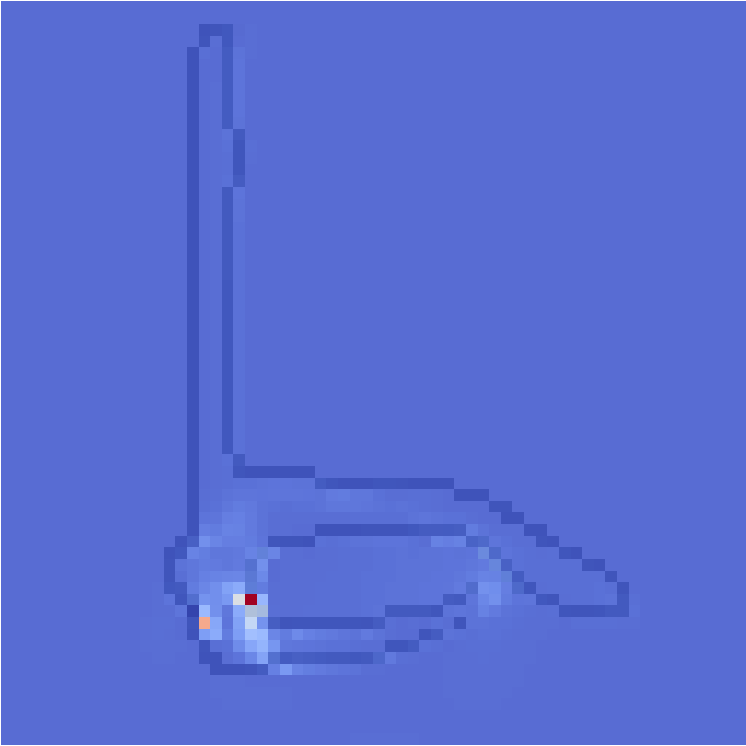
\includegraphics[width=1.5cm,height=1.5cm]{figs/ablation/pp-wo-27054.png}\hspace{0.2cm}
    
\includegraphics[width=1.5cm,height=1.5cm]{figs/ablation/27054-wo-pe.png}\hspace{0.02cm}
    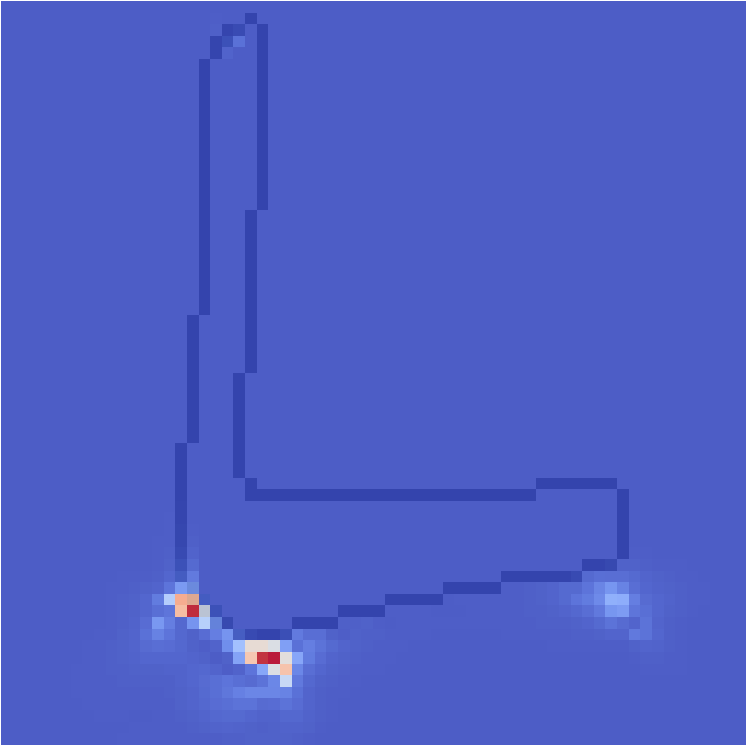
\includegraphics[width=1.5cm,height=1.5cm]{figs/ablation/pe-wo-27054.png}\hspace{0.2cm}
    
\includegraphics[width=1.5cm,height=1.5cm]{figs/ablation/27054-wo-pf.png}\hspace{0.02cm}
    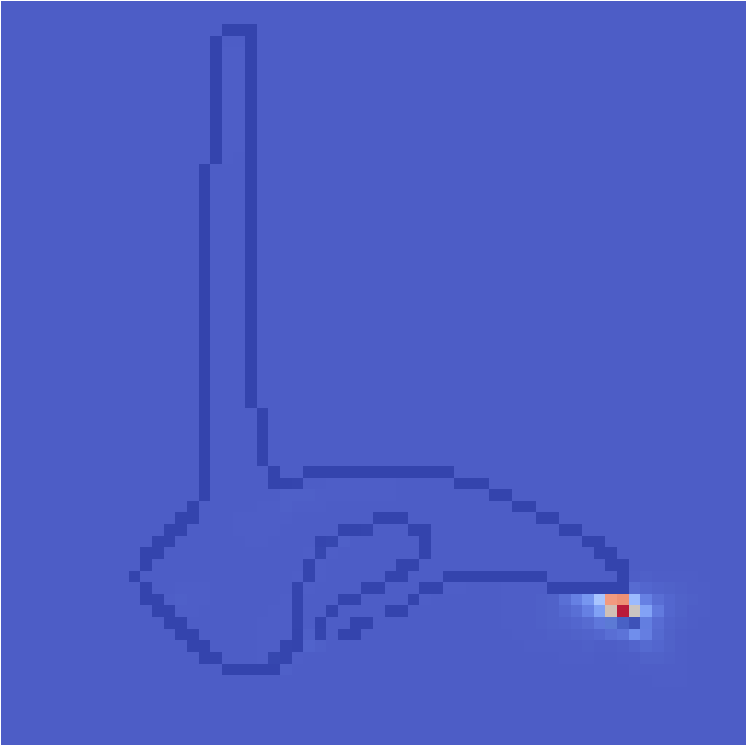
\includegraphics[width=1.5cm,height=1.5cm]{figs/ablation/pf-wo-27054.png}
    % \vspace{-1pt}
    \\
    \footnotesize{
    \makebox[1.5cm]{$\overline{V}=12.4\%$}\hspace{0.2cm}
    \makebox[1.5cm]{$vol=12.5\%$}\hspace{0.02cm}
    \makebox[1.5cm]{$comp=7.37e2$}\hspace{0.2cm}
    \makebox[1.5cm]{$vol=12.4\%$}\hspace{0.02cm}
    \makebox[1.5cm]{$comp=3.08e3$}\hspace{0.2cm}
    \makebox[1.5cm]{$vol=12.9\%$}\hspace{0.02cm}
    \makebox[1.5cm]{$comp=6.85e4$}
    \makebox[1.5cm]{$vol=12.5\%$}\hspace{0.02cm}
    \makebox[1.5cm]{$comp=6.32e3$}}
    % \vspace{2pt}
    \\
    
\includegraphics[width=1.5cm,height=1.5cm]{figs/ablation/27071-gt.png}\hspace{0.2cm}
    
\includegraphics[width=1.5cm,height=1.5cm]{figs/ablation/27071-pred.png}\hspace{0.02cm}
    
\includegraphics[width=1.5cm,height=1.5cm]{figs/ablation/strain-27071.png}\hspace{0.2cm}
    
\includegraphics[width=1.5cm,height=1.5cm]{figs/ablation/27071-wo-pp.png}\hspace{0.02cm}
    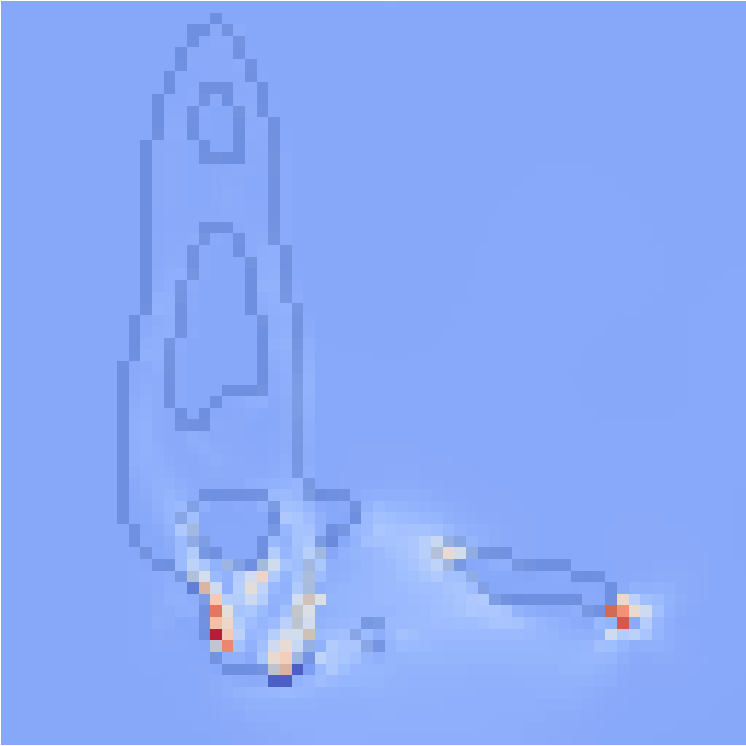
\includegraphics[width=1.5cm,height=1.5cm]{figs/ablation/pp-wo-27071.png}\hspace{0.2cm}
    
\includegraphics[width=1.5cm,height=1.5cm]{figs/ablation/27071-wo-pe.png}\hspace{0.02cm}
    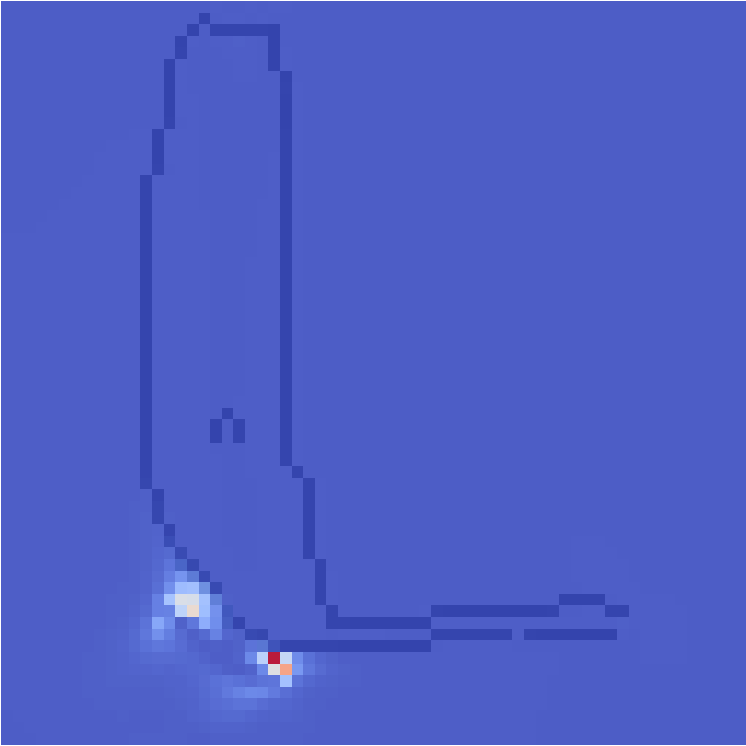
\includegraphics[width=1.5cm,height=1.5cm]{figs/ablation/pe-wo-27071.png}\hspace{0.2cm}
    
\includegraphics[width=1.5cm,height=1.5cm]{figs/ablation/27071-wo-pf.png}\hspace{0.02cm}
    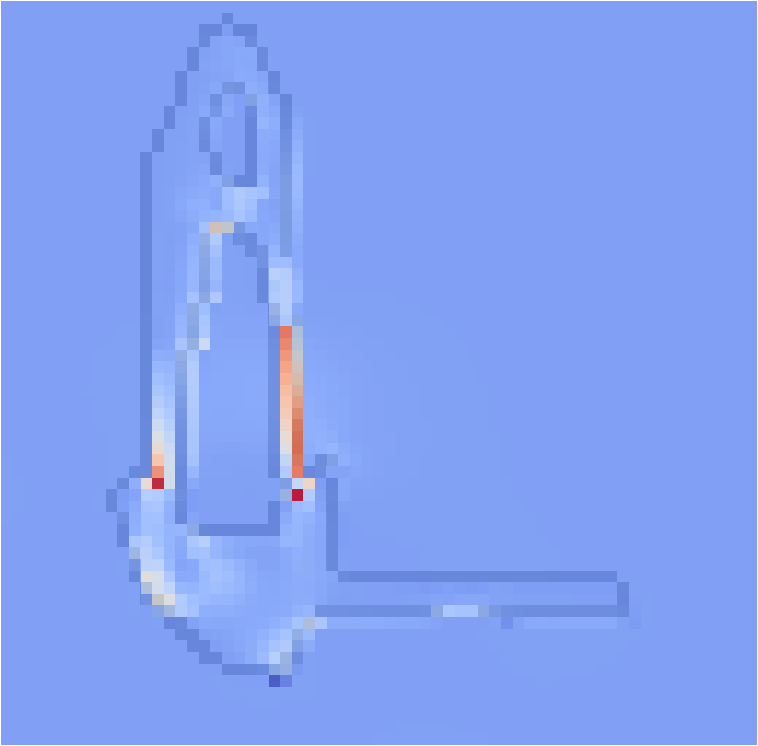
\includegraphics[width=1.5cm,height=1.5cm]{figs/ablation/pf-wo-27071.png}
    % \vspace{-1pt}
    \\
    \footnotesize{
    \makebox[1.5cm]{$\overline{V}=15.0\%$}\hspace{0.2cm}
    \makebox[1.5cm]{$vol=15.0\%$}\hspace{0.02cm}
    \makebox[1.5cm]{$comp=8.30e3$}\hspace{0.2cm}
    \makebox[1.5cm]{$vol=12.57\%$}\hspace{0.02cm}
    \makebox[1.5cm]{$comp=2.59e4$}\hspace{0.2cm}
    \makebox[1.5cm]{$vol=15.6\%$}\hspace{0.02cm}
    \makebox[1.5cm]{$comp=3.11e5$}
    \makebox[1.5cm]{$vol=12.5\%$}\hspace{0.02cm}
    \makebox[1.5cm]{$comp=9.34e3$}}
    % \vspace{2pt}
    \\
    
\includegraphics[width=1.5cm,height=1.5cm]{figs/ablation/3096-gt.png}\hspace{0.2cm}
    
\includegraphics[width=1.5cm,height=1.5cm]{figs/ablation/3096-pred.png}\hspace{0.02cm}
    
\includegraphics[width=1.5cm,height=1.5cm]{figs/ablation/strain-3096.png}\hspace{0.2cm}
    
\includegraphics[width=1.5cm,height=1.5cm]{figs/ablation/3096-wo-pp.png}\hspace{0.02cm}
    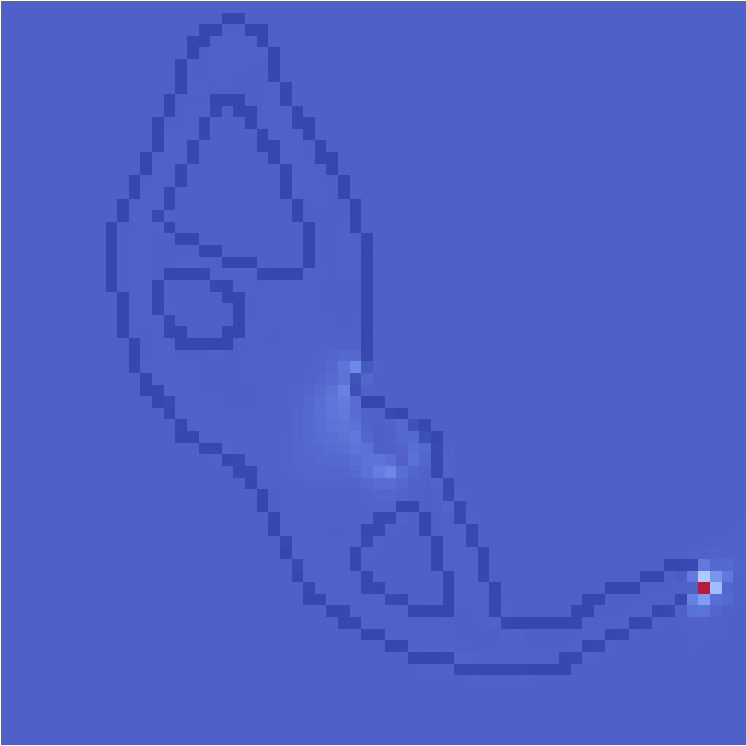
\includegraphics[width=1.5cm,height=1.5cm]{figs/ablation/pp-wo-3096.png}\hspace{0.2cm}
    
\includegraphics[width=1.5cm,height=1.5cm]{figs/ablation/3096-wo-pe.png}\hspace{0.02cm}
    
\includegraphics[width=1.5cm,height=1.5cm]{figs/ablation/pe-wo-3096.png}\hspace{0.2cm}
    
\includegraphics[width=1.5cm,height=1.5cm]{figs/ablation/3096-wo-pf.png}\hspace{0.02cm}
    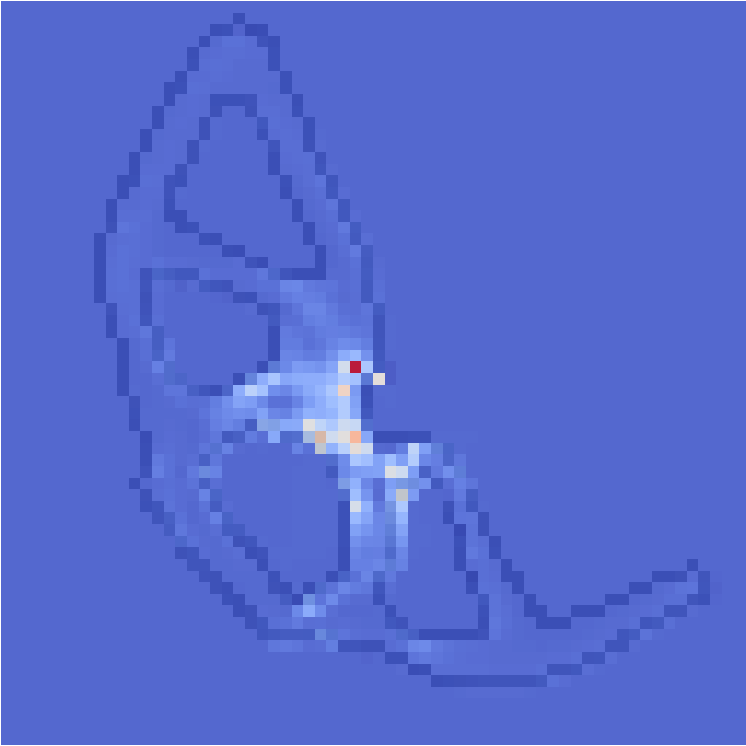
\includegraphics[width=1.5cm,height=1.5cm]{figs/ablation/pf-wo-3096.png}
    % \vspace{-1pt}
    \\
    \footnotesize{
    \makebox[1.5cm]{$\overline{V}=20.0\%$}\hspace{0.2cm}
    \makebox[1.5cm]{$vol=18.9\%$}\hspace{0.02cm}
    \makebox[1.5cm]{$comp=3.25e3$}\hspace{0.2cm}
    \makebox[1.5cm]{$vol=18.9\%$}\hspace{0.02cm}
    \makebox[1.5cm]{$comp=4.85e3$}\hspace{0.2cm}
    \makebox[1.5cm]{$vol=18.9\%$}\hspace{0.02cm}
    \makebox[1.5cm]{$comp=5.38e3$}
    \makebox[1.5cm]{$vol=18.9\%$}\hspace{0.02cm}
    \makebox[1.5cm]{$comp=6.01e3$}}
    \end{graybox}
    \small{
    \resizebox{0.66\textwidth}{!}{\begin{tabular}{lcccc}
        \toprule
        \textbf{Metrics}                     & \textbf{IF-TONIR} & \textbf{w/o point properties} & \textbf{w/o positional encoding} &\textbf{w/o physical fields} \\
        \midrule
        \textbf{Average $\epsilon^{comp}$} & $54.2\%$                    & $296.9\%$ & $114.8\%$ & $208.4\%$  \\
        \midrule
        \textbf{Average $\epsilon^{vol}$}                            & $4.02\%$                & $5.85\%$   & $5.33\%$ & $5.20\%$  \\
        \bottomrule
    \end{tabular}}}
    \caption{Comparative results illustrating the importance of local network architecture. Columns 2-3 show the optimized structure and corresponding strain energy field of the complete network framework; Columns 4-5 depict the results without point properties; Columns 6-7 present the results without positional encoding; Columns 8-9 display the results after removing stress and strain energy fields from the physical information.}
    \label{fig:ablation}
\end{figure}